\documentclass[10.5pt,twocolumn]{jbuaa}
\usepackage[noend]{algpseudocode}
\usepackage{amsmath}
\usepackage{booktabs}
\usepackage{algorithm}
\newcommand*\circled[1]{\tikz[baseline=(char.base)]{
            \node[shape=circle,draw,inner sep=1pt] (char) {#1};}}
\usepackage{amsmath}  
\usepackage{float}   
\usepackage[numbered,framed, autolinebreaks]{mcode}
%取消英文连词符
% \tolerance=1
% \emergencystretch=\maxdimen
% \hyphenpenalty=10000
% \hbadness=10000
\usepackage{enumitem}
\usepackage{bm}
\renewcommand{\algorithmicrequire}{\textbf{Input:}}
\renewcommand{\algorithmicensure}{\textbf{Output:}}
\newcommand{\horrule}[1]{\rule{\linewidth}{#1}} % Create horizontal rule command with 1 argument of height
\newcommand\mycolorRed[1]{{\color{red}#1}}
\newcommand\mycolorYellow[1]{{\color{yellow}#1}}
% \newcommand*\mycolorRed{\color{red}}

%%%????? 公式中字体的定义尺寸为 10 磅,上标/下标 68%,次下标/上标 42% ?????? 
\DeclareMathSizes{10.5}{10}{6.8}{4.2}
%%%% 本示例中带单位的数据采用的是siunitx来生成,好像默认与公式同样大小的字体,所以数字在正文中会小一些
%%%% 行文中普通数字大小为10.5pt,公式里或者用siunitx生成的数字则会是10pt,多少有点不协调。

%%%设置公式前后距离,差不多近似
\setlength{\abovedisplayskip}{2.5mm}
\setlength{\belowdisplayskip}{2.5mm}


\usepackage{tabu}
\usepackage{longtable}
\usepackage{makecell}
\renewcommand\cellgape{\Gape[-3pt][-3pt]}


%%%%%%%%%%%%%%%%%%%%%%%%%%%%%%%%%%%%%%%%%%%%%%%%%%%%%%%%%%%%%%%%
%      文章正文
%%%%%%%%%%%%%%%%%%%%%%%%%%%%%%%%%%%%%%%%%%%%%%%%%%%%%%%%%%%%%%%%
\begin{document}
%%%%%%%%%%%%%%%%%%%%%%%%%%%%%%%%%%%%%%%%%%%%%%%%%%%%%%%%%%%%%%%%
% 标题,基金项目,作者,通信地址定义
%%%%%%%%%%%%%%%%%%%%%%%%%%%%%%%%%%%%%%%%%%%%%%%%%%%%%%%%%%%%%%%%
\title{
\vspace{1cm} \erhao\hei 一个多节点声纳系统中同步时钟机制的可靠性评估和系统优化问题\vspace{-0.2cm}
}

\author{
\sihao\fang 吕艺 \makebox{$^{\text{1}}$},冯伟琪 \makebox{$^{\text{2}}$}\\[0.1cm]
\liuhao (1.~~上海交通大学~~电子信息电气工程学院,上海~~200240;2.~~上海交通大学~~电子信息电气工程学院,上海~~200240)
}

\date{}  % 这一行用来去掉默认的日期显示
%%%%%%%%%%%%%%%%%%%%%%%%%%%%%%%%%%%%%%%%%%%%%%%%%%%%%%%%%%%%%%%%
% 奇数页页眉
%%%%%%%%%%%%%%%%%%%%%%%%%%%%%%%%%%%%%%%%%%%%%%%%%%%%%%%%%%%%%%%%
\fancyhead[CO]{{\footnotesize 工程建模与仿真}}            %请在这里写出第一作者以及论文题目
%%%%%%%%%%%%%%%%%%%%%%%%%%%%%%%%%%%%%%%%%%%%%%%%%%%%%%%%%%%%%%%%
%%%%%%%%%%%%%%%%%%%%%%%%%%%%%%%%%%%%%%%%%%%%%%%%%%%%%%%%%%%%%%%%
%  显示title,并设页码为空(按杂志社要求)
%%%%%%%%%%%%%%%%%%%%%%%%%%%%%%%%%%%%%%%%%%%%%%%%%%%%%%%%%%%%%%%%
%%%%%%%%%%%%%%%%%%%%%%%%%%%%%%%%%%%%%%%%%%%%%%%%%%%%%%%%%%%%%%%%
%      中文摘要
%%%%%%%%%%%%%%%%%%%%%%%%%%%%%%%%%%%%%%%%%%%%%%%%%%%%%%%%%%%%%%%%
\CKeyword{多节点声呐系统;蒙特卡洛算法;马尔科夫链;可靠性估算}
\twocolumn[
  \begin{@twocolumnfalse}
  \maketitle
\begin{CAbstractJBUAA}
本文首先引入了一个多节点声呐系统中同步时钟机制的可靠性评估和系统优化问题,并且构建了相应的理论模型。然后,本文介绍了蒙特卡洛算法的基本思想和马尔科夫链的数学内涵。针对案例中的优化问题,本文提出了两种蒙特卡洛随机模拟算法,并且对两种算法对应的模拟效果进行对比分析。最后,我们利用蒙特卡洛模拟算法解决了最优系统升级方案问题。
\end{CAbstractJBUAA}
\begin{center}
\parbox{\textwidth}{
\setlength{\parindent}{1em}
{
\centering\sihao\textbf{Reliability Evaluation and System Optimization Problem of Synchronous Clock Mechanism in a Multi-Node Sonar System}\\
} 
\vspace{-1.2mm}
\begin{center}
\wuhao Yi Lyu\makebox{$^{\text{1}}$}, Vic Feng\makebox{$^{\text{2}}$}\\[-0.1cm]
\liuhao{1. School of Electrical and Engineering, Shanghai Jiao Tong University, Shanghai 200240, China;\\
2. School of Electrical and Engineering, Shanghai Jiao Tong University, Shanghai 200240, China;}
\end{center}

\wuhao
{
\textbf{Abstract:} 
Initially, a reliability evaluation and optimization problem of a multi-node sonar system is carried out, for which a corresponding theoretical model is built. In addition, we introduce the basic ideas and mathematical theories of Markov chain Monte Carlo. For optimization problem, we tried two MCMC algorithms and then compared them by their performances. Finally, we solved the best system optimization problem by applying MCMC simulation algorithm.

\textbf{Key words:} Multi-node sonar system; Monte Carlo algorithm; Markov chain; Reliability evaluation}
}
\end{center}

  \end{@twocolumnfalse}
]
%%%%%%%%%%%%%%%%%%%%%%%%%%%%%%%%%%%%%%%%%%%%%%%%%%%%%%%%%%%%%%%%
%  正文由此开始-------------------------
%%%%%%%%%%%%%%%%%%%%%%%%%%%%%%%%%%%%%%%%%%%%%%%%%%%%%%%%%%%%%%%%
%%%%%%%%%%%%%%%%%%%%%%%%%%%%%%%%%%%%%%%%%%%%%%%%%%%%%%%%%%%%%%%%
\wuhao 
\section{引言}
\subsection{课题背景\cite{cite1}}
某分布式部署的声纳系统共有$n$个独立节点构成。各节点内部均是物理同构的。各节点必须保持严格的时钟信号同步才能有效协同工作,使系统发挥作用。所有节点经由时钟信号总线连接,由其中一个节点担当主节点,它的时钟电路工作于主模式,向总线输出时钟信号; 其余节点均应担当从节点,节点内部时钟电路工作于从模式,仅从总线获取信号,不向总线输出信号。节点可能发生故障。由于应用场合的特殊性,故障一旦发生就无法修复。
\subsection{问题求解}
根据前理论假设、基本参数和理论模型,确立仿真算法,用蒙特卡洛法模拟$S$套同型系统的运行状况。建议取 $S \geq 10000$。

系统的可靠性统计式如公式\eqref{eq:1}所示:

\begin{equation}
	R(w) = \sum_{i = 1}^{S}1(T_f^{(i)} \geq w) / s
	\label{eq:1}
\end{equation}

其中$T_f^{(i)}$为仿真实验的$S$套声纳系统中第$i$套的有效工作寿命。

\begin{enumerate}
	\item 通过随机模拟运行实验,求节点总数n,使系统可靠性 最大$R(w)|_{w = 25000h}$最大,其中$n = 4, 5, \cdots, 12$
	\item 通过随机模拟运行试验,求节点数$n$,使系统平均工作寿命$E(T_f)$最大,其中$n = 4, 5, \cdots, 12$。
\end{enumerate}
\section{理论假设及模型建立\cite{cite1}}
\subsection{模型元件与部件}
 模型元件与部件
我们将切换器$A$和切换器$B$视作不可靠元件,而将系统中的其余元件均视作不失效的可
靠元件,这些元件的失效风险已被等效地折算计入不可靠元件的失效风险中。 

切换器可视作一种多状态元件,且彼此特性统计独立。由各元件组成的节点是构成系统
的部件,显然其性能表现也是多状态的。声纳系统整体可看作一个多状态系统。
\subsection{理论假设及参数}
\subsubsection{切换器A的故障类型与概率}
切换器$A$可能出现3种类型的故障,分别称为$A1$、$A2$、$A3$。

切换器$A$使用寿命$T_A$的概率密度分布为$f_{T_A}(\tau) = \lambda_A e^{-\lambda_A \tau}$,其中$\frac{1}{\lambda_A} = 9.55 \times 10 ^ 4\ hour$。
\begin{enumerate}
	\item 故障$A1$: 掷刀无法与触点1脱离。$P_{EA1} = Pr(A1\   occurs | A
	  \ is\ failed) = 0.23$
	\item 故障$A2$: 掷刀无法与触点1脱离。$P_{EA1} = Pr(A2\ occurs | A\ is\ failed) = 0.27$
	 \item 故障$A3$: 掷刀无法与触点1脱离。$P_{EA1} = Pr(A3\ 
	  occurs | A\ 
	  is\ failed) = 0.50$
\end{enumerate}
\subsubsection{切换器B的故障类型与概率}
切换器$B$可能出现2种类型的故障,分别称作$B1$、$B2$。

切换器$B$使用寿命$T_B$的概率密度分布$f_{T_B}(\tau) = \lambda_B e^{-\lambda_B \tau}$。其中$\frac{1}{\lambda_B} = 2.9 \times 10^ 5 hour$。
\begin{enumerate}
	\item 故障$B1$: 掷刀无法与触点脱离。$P_{EB1} = Pr(B1\ occurs | B\ is\ failed) = 0.73$
	\item 故障$B2$:掷刀无法与触点接合。$P_{EB2} = Pr(B2\ occurs | B\ is\ failed) = 0.27$
\end{enumerate}
\subsubsection{其他理论假设}
\begin{enumerate}
	\item 不同元件随机状态的统计特性彼此独立
	\item 元件一旦发生故障,故障类型即刻确定,且其后不会发生变化
	\item 故障均不可修复
	\item 本课题$k$取定值4。
\end{enumerate}
\subsection{模型建立}
从整体性能的角度,我们可以将整个系统的状态归为4类,$G_{sys}(t)\in \{G_{sys1}, G_{sys2}, G_{sys3}, G_{sys4}\}$。下文中提到条件$C_i (i = 1, 2, \cdots , 9)$的具体内容,参见指导文献\cite{cite1}。
\begin{enumerate}
	\item 系统确定不能有效工作的状态$G_{sys1}$:\quad $G_{sys1} = C1\ ||\ C2 ||\ C3 \ || \ C4$。
	\item 系统确定能有效工作的状态$G_{sys2}$:\quad $G_{sys2} = C5 \cap (C6 \cup C7)$
	\item 同时满足条件$C8$和$C9$,系统恰能有效工作的状态$G_{sys3}$:当$G_{sys3} = C8 \cap C9$时,系统在一定概率下有效工作。只有当任一个处于$g_{DM}$的节点恰好被选作主节点时。系统有效节点总数才能达到$k$,恰好可以有效工作,称为状态$G_{sys3}$
	\item 同时满足条件$C8$和$C9$,系统恰不能有效工作的状态$G_{sys4}$:当同时满足条件$C8$和$C9$,而任一个处于$g_{PF}$的节点被选作主节点使,系统有效节点总数只能达到$k - 1$,恰好不能有效状态,称为状态$G_{sys4}$。
\end{enumerate}
\section{算法设计}
案例背景为一个可靠性计算问题,我们可以采用\textbf{概率统计理论推算}和\textbf{蒙特卡洛模拟}两种算法进行求解。由于理论推算算法相对繁琐,我们放在自主探究一节进行进一步讨论。这里我们利用简单清晰的蒙特卡洛算法进行随机模拟。
\subsection{算法思想}
首先,我们对\textbf{蒙特卡洛算法}进行简要介绍。\textbf{蒙特卡罗算法}是一种以概率和统计理论方法为基础的一种模拟方法。\textbf{蒙特卡洛算法}将所求解的问题同一定的概率模型相联系,用电子计算机实现统计模拟或抽样,以获得问题的近似解\cite{cite2}。 在本案例中,由于元件的寿命服从一定的指数分布。因此,指数分布即为本案例背景下的概率模型。

为了证明算法的正确性,我们还需引入一个特别的随机过程形式 —— \textbf{马尔科夫链}。考虑到马尔科夫链的复杂性,我们仅引入马尔科夫链的离散形式\cite{cite4}。 假设随机过程$X(t)$的取值为离散,比如$X(t) \in \{1, 2, \cdots \}$,如果对$t_1 < t_2 < \cdots < t_{n - 1} < t_{n}$,$X(t)$的条件概率函数满足等式\eqref{eq:2}:
\begin{equation} \label{eq:2}
\begin{split}
	Pr
	\{X(t_n) = x_n  | X(t_{n - 1}), \cdots,  X(t_1) = x_1\}
	\\
	  = Pr\{X(t_n) = x_n | X(t_{n - 1}) = x_{n - 1}\}
\end{split}
\end{equation}

即在$X(t_{n - 1})$确定的情况下,$X(t_n)$的取值不依赖于$t_{n - 1}$之前时刻的取值,则称如上随机过称为马尔科夫链。

根据理论分析可知,我们发现马尔科夫链无后效性,指数分布无记忆性。因此我们可以根据马尔科夫链设计第一种算法,按时间定步长推进。虽然元件的使用寿命在时间轴上是连续的,但我们为了利用马尔科夫链的离散形式对时间进行离散化。我们取时间推动步长为1小时,在时刻$t$时整个系统的状态转换过程可以利用图1中的有限状态机($FSM$)进行模拟示意。考虑到马尔科夫链的无后效性,我们发现每一时刻$t$的状态转移矩阵$P$完全相同。因此采用定时间步长进行随机模拟的算法是正确可行的。

\begin{figure}[H]
\centering
	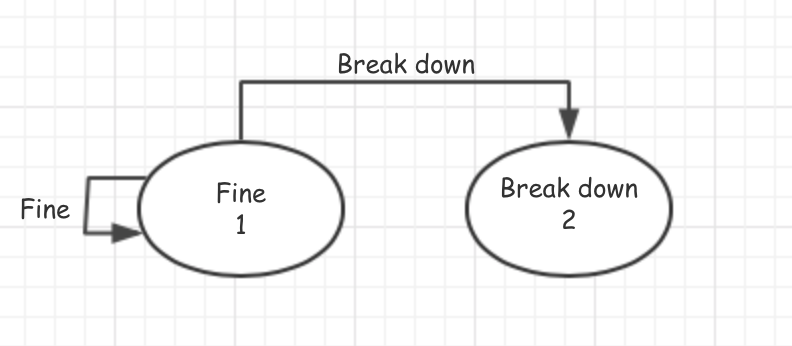
\includegraphics[scale = 0.5]{fig1}
	\caption{系统在时刻$t$的有限状态机示意图}
\end{figure}

由于按定步长推动时间变化算法的效率较低,我们考虑采用变步长推动时间变化。如果人为确定变化步长的策略,我们可能会\textbf{错过}系统失效的节点,从而增大我们随机模拟得到的系统平均寿命。因此,我们需要一种合理恰当的变步长模拟方法。

我们重新考虑到前文提到的马尔科夫链的无后效性,当前时刻的工作状态仅与上一时刻有关。因此,我们可以从一开始就确定所有元件的寿命(符合一定的指数分布),这与按一定步长推进时间来估算系统是否损坏是等效的。采用这种方法,我们可以大大减少整个算法的时间复杂度。只需每次根据不同元件的使用寿命,寻找当前使用寿命最小的元件,考虑它的损坏对整个系统的影响。由于其与定步长随机模拟算法的等效性,因此该变步长算法也是正确的。其具体算法实现将在下一小节以程序框图的形式具体表现。
\subsection{算法实现与程序框图}
首先,我们给出定步长的算法实现。根据上一小节和指导文献\cite{cite1}的提示,我们选择步长为1小时,最大时间为75000小时。其程序框图如图\ref{fig:2} 所示:
\begin{figure}[H]
	\centering
	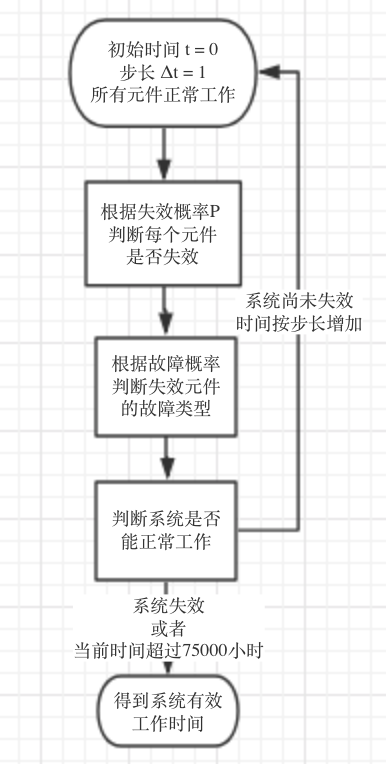
\includegraphics{fig2}
	\caption{定步长蒙特卡洛算法流程图}
	\label{fig:2}
\end{figure}
根据程序框图\ref{fig:2},定步长蒙特卡洛算法简单清晰。通过将时间离散化,按照一定步长在不同时刻确定整个系统的状态。但从另一个角度来看,该算法的时间复杂性相对较高。每套系统的模拟必须遍历所有可能的时间节点,这极大的增加模拟所需的时间成本。而第二种变步长蒙特卡洛模拟算法则会完美解决这一点。

第二种变步长蒙特卡洛模拟算法的主要思想在上一小节中已经具体阐述。其值得注意的一点是由于最大时间$T_{max}$的存在,我们需要对使用寿命超过$T_{max}$的系统进行\textbf{截尾}操作,将其寿命赋值为最大时间。其程序框图如图\ref{fig:3} 所示:

\begin{figure}[H]
	\centering
	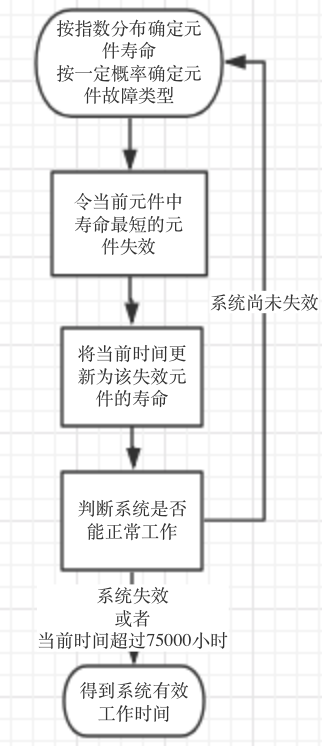
\includegraphics{fig3}
	\label{fig:3}
	\caption{变步长蒙特卡洛算法流程图}
\end{figure}

变步长蒙特卡洛算法拥有卓越的性能体现,大规模模拟仿真所需要的时间远远小于利用定步长蒙特卡洛算法所需要的时间。其算法实现相较于蒙特卡洛算法更加简洁迅速,并且有着不俗的性能表现。在下一小节中,我们会对两种算法的实际仿真效果进行进一步分析和比较。
\section{仿真结果对比及分析}
在这一小节中,我们分别利用两种蒙特卡洛方法针对节点个数$n$的不同取值,进行模拟仿真试验。
\subsection{定步长蒙特卡洛算法试验结果}
利用定步长蒙特卡洛算法,我们对$S = 10000$组系统进行随机模拟实验。系统最大可靠性在$n = 7$时取得,系统在$n = 6, 7, 8, 9$时都可能取得较大的系统可靠性;系统平均寿命在$n = 8$时取得最大值,系统在$n = 7, 8, 9$时都可取得较大的系统平均寿命。其具体模拟仿真数据如表\ref{table:1} 所示:
\begin{table}[H]
	\centering
	\label{table:1}
	\caption{定步长蒙特卡洛算法模拟仿真结果}
	\vspace{0.2cm}
	\begin{tabular}{c|c|c|c}
	\hline
	n & \kai 系统可靠性 & \kai 系统平均寿命(h) & \kai 计算时间(s) \\
	\hline
	4 & 0.474 & 29888 & 120.02\\
	\hline
	5 & 0.776 & 47382 & 145.26\\
	\hline
	6 & 0.889 & 56221 & 179.80\\
	\hline
	7 & 0.915 & 59777 & 202.12\\
	\hline
	8 & 0.909 & 60446 & 233.22\\
	\hline
	9 & 0.897 & 59843 & 255.66\\
	\hline
	10 & 0.879 & 58392 & 277.01\\
	\hline
	11 & 0.859 & 56541 & 299.12\\
	\hline
	12 & 0.837 & 54779 & 328.99\\
	\hline
		
	\end{tabular}
\end{table}

为了直观的展现数据趋势,我们分别以节点个数$n$为横坐标,以系统可靠性和系统平均寿命为纵坐标,绘制相关折线图如图\ref{fig:4}和图\ref{fig:5} 所示。
\begin{figure}[H]
	\centering
	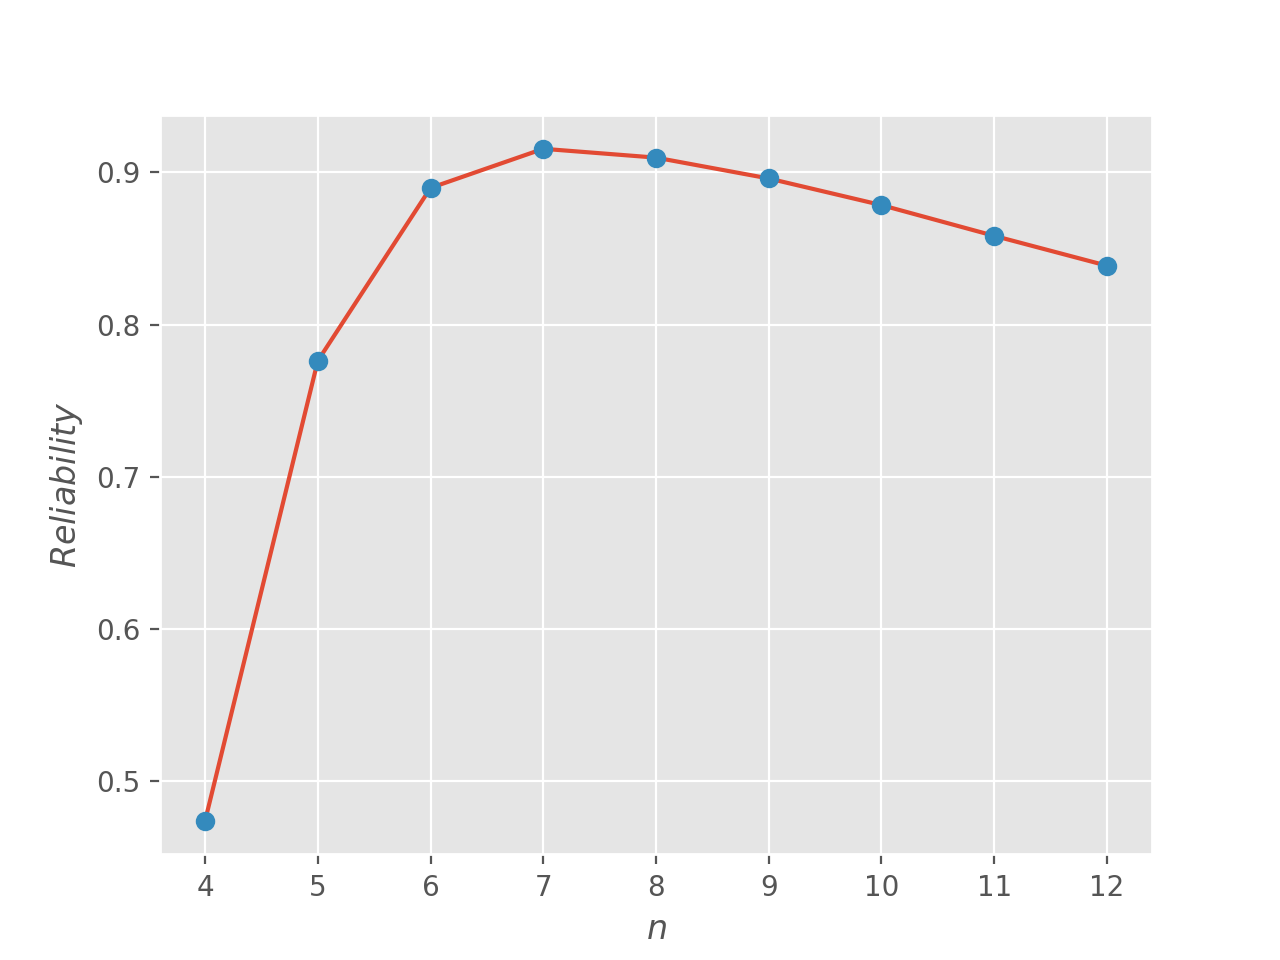
\includegraphics[scale = 0.6]{fig4}
	\caption{系统可靠性和节点个数关系示意图}
	\label{fig:4}
\end{figure}

\begin{figure}[H]
	\centering
	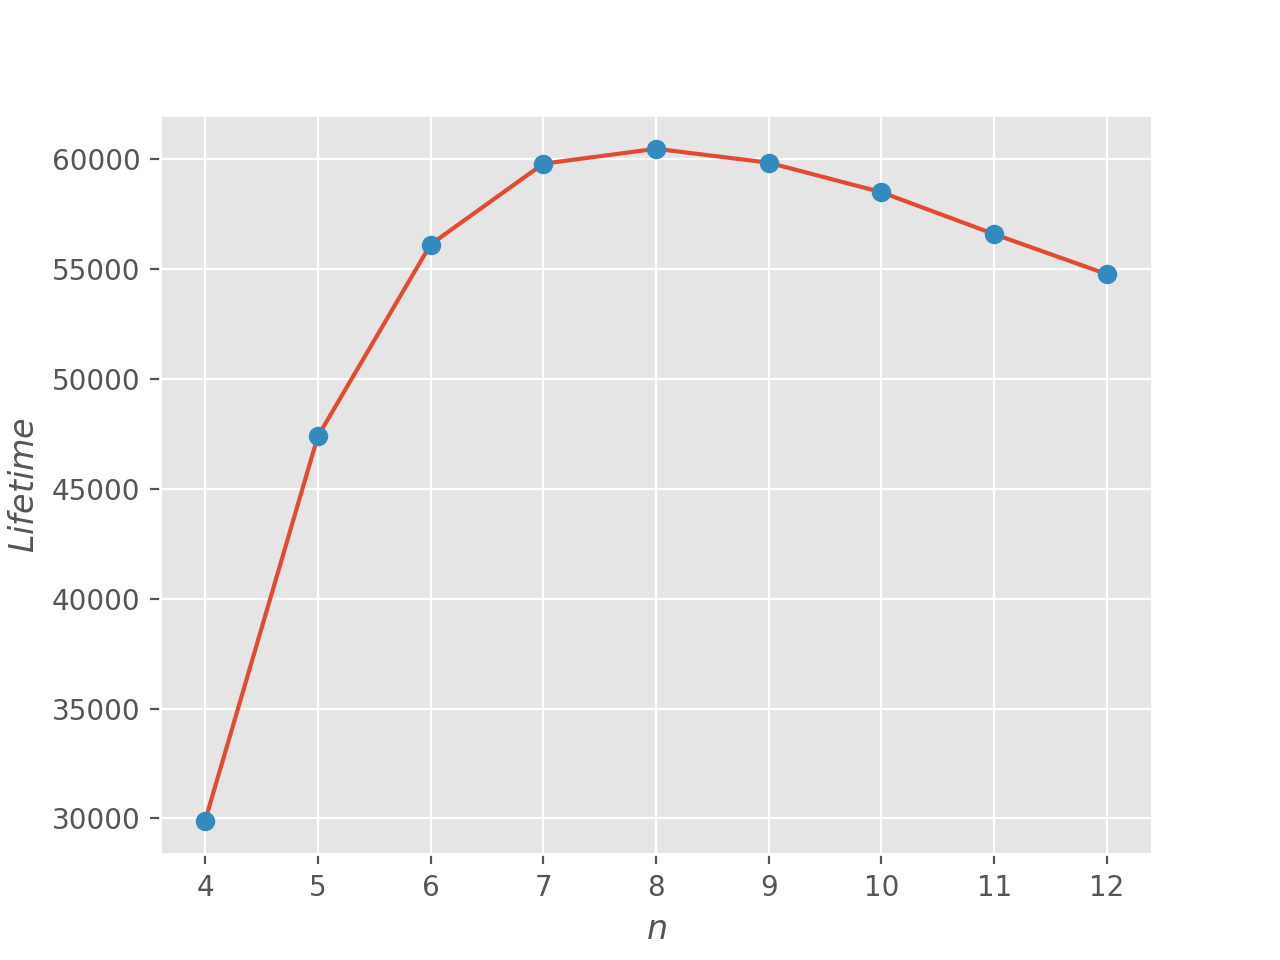
\includegraphics[scale = 0.6]{fig5}
	\caption{系统平均寿命和节点个数关系示意图}
	\label{fig:5}
\end{figure}
\subsection{变步长蒙特卡洛算法试验结果}
利用变步长蒙特卡洛算法,我们对$S = 10000$组系统进行随机模拟试验。系 统 最 ⼤ 可 靠 性 在 $n = 7$ 时 取 得, 系 统 在 $n = 6, 7, 8, 9$ 时 都 可 能 取 得 较 ⼤ 的 系 统 可 靠 性; 系 统 平 均 寿 命 在 $n = 8$ 时 取 得 最 ⼤ 值, 系 统 在 $n = 7, 8, 9$ 时 都 可 取 得 较 ⼤ 的系统平均寿命。其具体模拟仿真数据如表\ref{table:2} 所⽰
\begin{table}[H]
	\centering
	\label{table:2}
	\caption{变步长蒙特卡洛算法模拟仿真结果}
	\vspace{0.2cm}
	\begin{tabular}{c|c|c|c}
	\hline
	n & \kai 系统可靠性 & \kai 系统平均寿命(h) & \kai 计算时间(s) \\
	\hline
	4 & 0.478 & 29897 & 12.82\\
	\hline
	5 & 0.774 & 47281 & 14.16\\
	\hline
	6 & 0.887 & 56419 & 19.80\\
	\hline
	7 & 0.918 & 59768 & 20.12\\
	\hline
	8 & 0.906 & 60346 & 23.12\\
	\hline
	9 & 0.895 & 59828 & 24.76\\
	\hline
	10 & 0.876 & 58397 & 27.91\\
	\hline
	11 & 0.856 & 56531 & 29.63\\
	\hline
	12 & 0.834 & 54772 & 31.37\\
	\hline
		
	\end{tabular}
\end{table}
为了直观的展现数据趋势,我们分别以节点个数$n$为横坐标,以系统可靠性和系统平均寿命为纵坐标,绘制相关折线图如图\ref{fig:6}和图\ref{fig:7} 所示。
\begin{figure}[H]
	\centering
	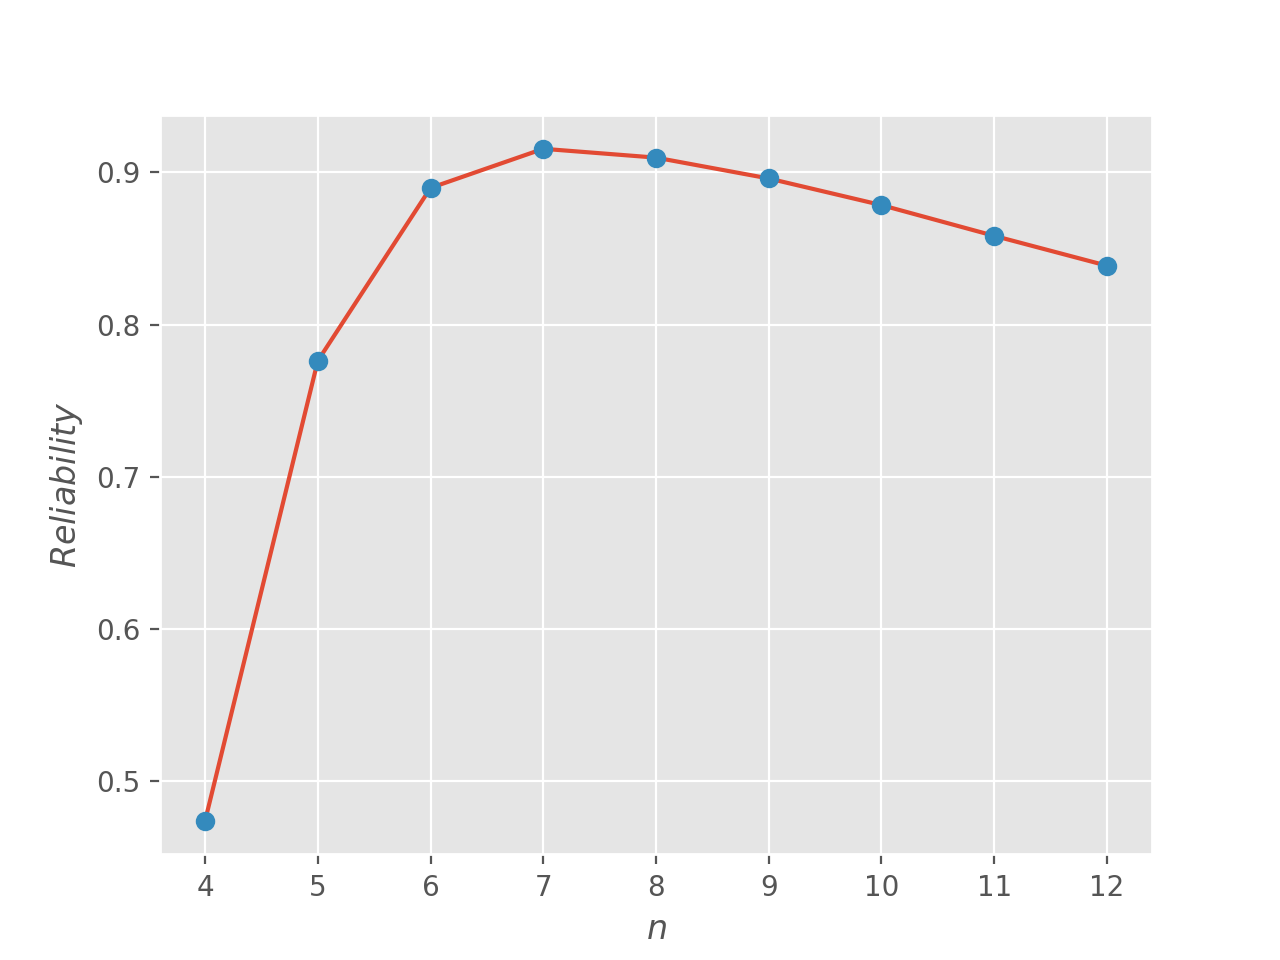
\includegraphics[scale = 0.6]{fig4}
	\caption{系统可靠性和节点个数关系示意图}
	\label{fig:6}
\end{figure}

\begin{figure}[H]
	\centering
	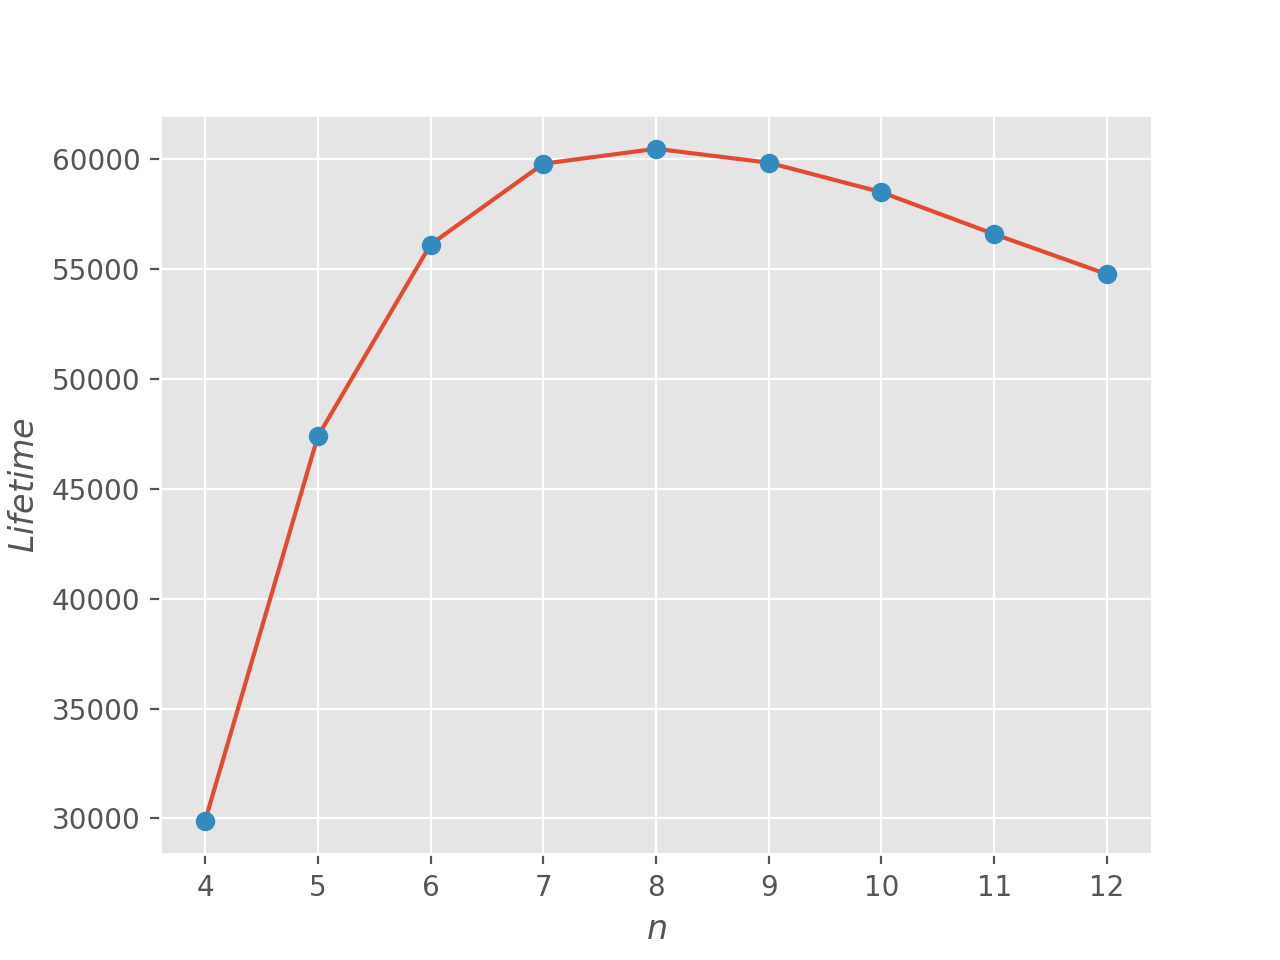
\includegraphics[scale = 0.6]{fig5}
	\caption{系统平均寿命和节点个数关系示意图}
	\label{fig:7}
\end{figure}

\subsection{两种算法结果对比及分析}
根据表\ref{table:1}和表\ref{table:2},我们可以发现两种算法的模拟结果基本完全相同。其主要区别点在时间效率上,变步长蒙特卡洛模拟算法显著优于定步长模拟算法。当节点$n$个数较多时,变步长的蒙特卡洛模拟算法有着约10倍的性能优势。在有限的时间性能和计算性能下,我们应当选择模拟效果较好的变步长蒙特卡洛算法,有限步长的蒙特卡洛算法有助于我们更好的理解整个仿真过程。
\section{自主探究}

\subsection{系统优化升级问题}
\textbf{探究问题:} 随着科学技术的不断进步,系统中的各个元件也会不断地升级换代。某公司决定对多节点声呐系统进行改造升级,提高元件的寿命。但碍于资金有限,某公司仅有三种改造方案:
\begin{enumerate}
	\item 升级所有元件中的$A$部件,使之寿命增加原来的一倍。
	\item 升级所有元件中的$B$部件,使之寿命增加原来的一倍。
	\item 同时升级元件中的$A, B$部件,但$A, B$部件的寿命均只能增加原来的一半。
\end{enumerate}

\textbf{求解思路:}利用变步长蒙特卡洛算法进行随机模拟试验,分别从可靠性和系统平均寿命两个指标选择最优方案。
\subsubsection{方案1}
根据方案1,我们升级所有元件中的$A$部件,使之寿命增加为原来的两倍。根据概率论中有关知识,我们可知部件$A$所服从指数分布的期望为原来的两倍。此时$\frac{1}{\lambda_A} = 1.91 \times 10 ^{5}\ hour$,我们对$S = 10000$组采用方案1升级的系统进行随机模拟。其模拟仿真结果如表\ref{table:3} 所示:
\begin{table}[H]
	\centering
	\label{table:3}
	\caption{方案1升级系统的模拟仿真结果}
	\vspace{0.2cm}
	\begin{tabular}{c|c|c}
	\hline
	n & \kai 系统可靠性 & \kai 系统平均寿命(h) \\
	\hline
	4 & 0.677 & 43455\\
	\hline
	5 & 0.891 & 59700 \\
	\hline
	6 & 0.938 & 64112 \\
	\hline
	7 & 0.932 & 64118 \\
	\hline
	8 & 0.918 & 62346 \\
	\hline
	9 & 0.901 & 60112 \\
	\hline
	10 & 0.879 & 58397 \\
	\hline
	11 & 0.856 & 56131 \\
	\hline
	12 & 0.838 & 54972 \\
	\hline
		
	\end{tabular}
\end{table}
\subsubsection{方案2}
根据方案2,我们升级所有元件中的$B$部件,使之寿命增加为原来的两倍。根据概率论中有关知识,我们可知部件$B$所服从指数分布的期望为原来的两倍。此时$\frac{1}{\lambda_B} = 5.8 \times 10 ^{5}\ hour$,我们对$S = 10000$组采用方案2升级的系统进行随机模拟。其模拟仿真结果如表\ref{table:4} 所示:
\begin{table}[H]
	\centering
	\label{table:4}
	\caption{方案2升级系统的模拟仿真结果}
	\vspace{0.2cm}
	\begin{tabular}{c|c|c}
	\hline
	n & \kai 系统可靠性 & \kai 系统平均寿命(h) \\
	\hline
	4 & 0.482 & 30455\\
	\hline
	5 & 0.792 & 49700 \\
	\hline
	6 & 0.928 & 59912 \\
	\hline
	7 & 0.958 & 65118 \\
	\hline
	8 & 0.968 & 67846 \\
	\hline
	9 & 0.961 & 67112 \\
	\hline
	10 & 0.955 & 67397 \\
	\hline
	11 & 0.945 & 66131 \\
	\hline
	12 & 0.940 & 66072 \\
	\hline
		
	\end{tabular}
\end{table}
\subsubsection{方案3}
根据方案3,我们同时升级所有元件中的$A, B$部件,使之寿命分别增加原来的一半。根据概率论中有关知识,此时$\frac{1}{\lambda_A} = 1.4325 \times 10 ^{5}\ hour$,$\frac{1}{\lambda_B} = 4.35 \times 10 ^{5}\ hour$。我们对$S = 10000$组采用方案3升级的系统进行随机模拟。其模拟仿真结果如表\ref{table:5} 所示:
\begin{table}[H]
	\centering
	\label{table:5}
	\caption{方案3升级系统的模拟仿真结果}
	\vspace{0.2cm}
	\begin{tabular}{c|c|c}
	\hline
	n & \kai 系统可靠性 & \kai 系统平均寿命(h) \\
	\hline
	4 & 0.607 & 38455\\
	\hline
	5 & 0.871 & 57700 \\
	\hline
	6 & 0.948 & 64812 \\
	\hline
	7 & 0.959 & 67018 \\
	\hline
	8 & 0.954 & 67146 \\
	\hline
	9 & 0.946 & 66312 \\
	\hline
	10 & 0.933 & 64397 \\
	\hline
	11 & 0.926 & 63131 \\
	\hline
	12 & 0.913 & 62972 \\
	\hline
		
	\end{tabular}
\end{table}
\subsubsection{最优方案分析}
为了便于直观分析数据,我们首先以节点个数$n$为横轴,不同优化方案对应系统的可靠性为纵轴绘制关系折线图。其曲线图如图\ref{fig:6} 所示:
\begin{figure}[H]
	\label{fig:6}
	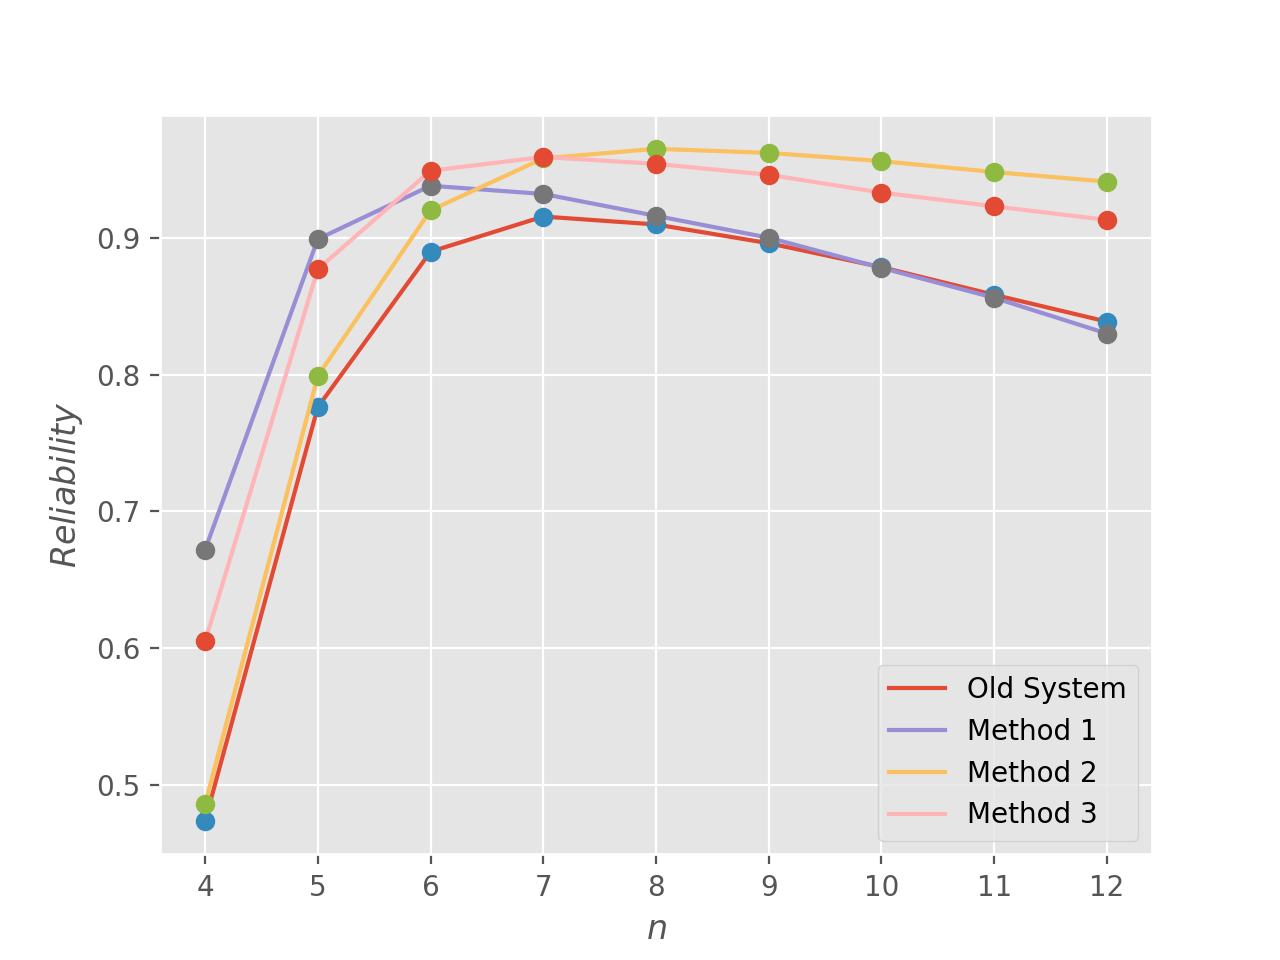
\includegraphics[scale = 0.6]{fig6}
	\caption{不同优化方案对应的可靠性和节点个数关系图}
\end{figure}

根据图\ref{fig:6}中不同曲线之间的相对关系,我们得出以系统可靠性为目标变量的最优方案选择标准。当$n < 6$时,我们应选择升级系统中所有元件中的部件$A$;当$ 6 \leq n \leq 8$时,我们应同时升级系统中所有元件中的部件$A$和部件$B$;当$ n > 8$时,我们应选择升级系统中所有元件的部件$B$。

然后我们再以节点个数$n$为横轴,不同优化方案对应系统的平均寿命为纵轴绘制关系折线图。其曲线图如图\ref{fig:7} 所示:

\begin{figure}[H]
	\label{fig:7}
	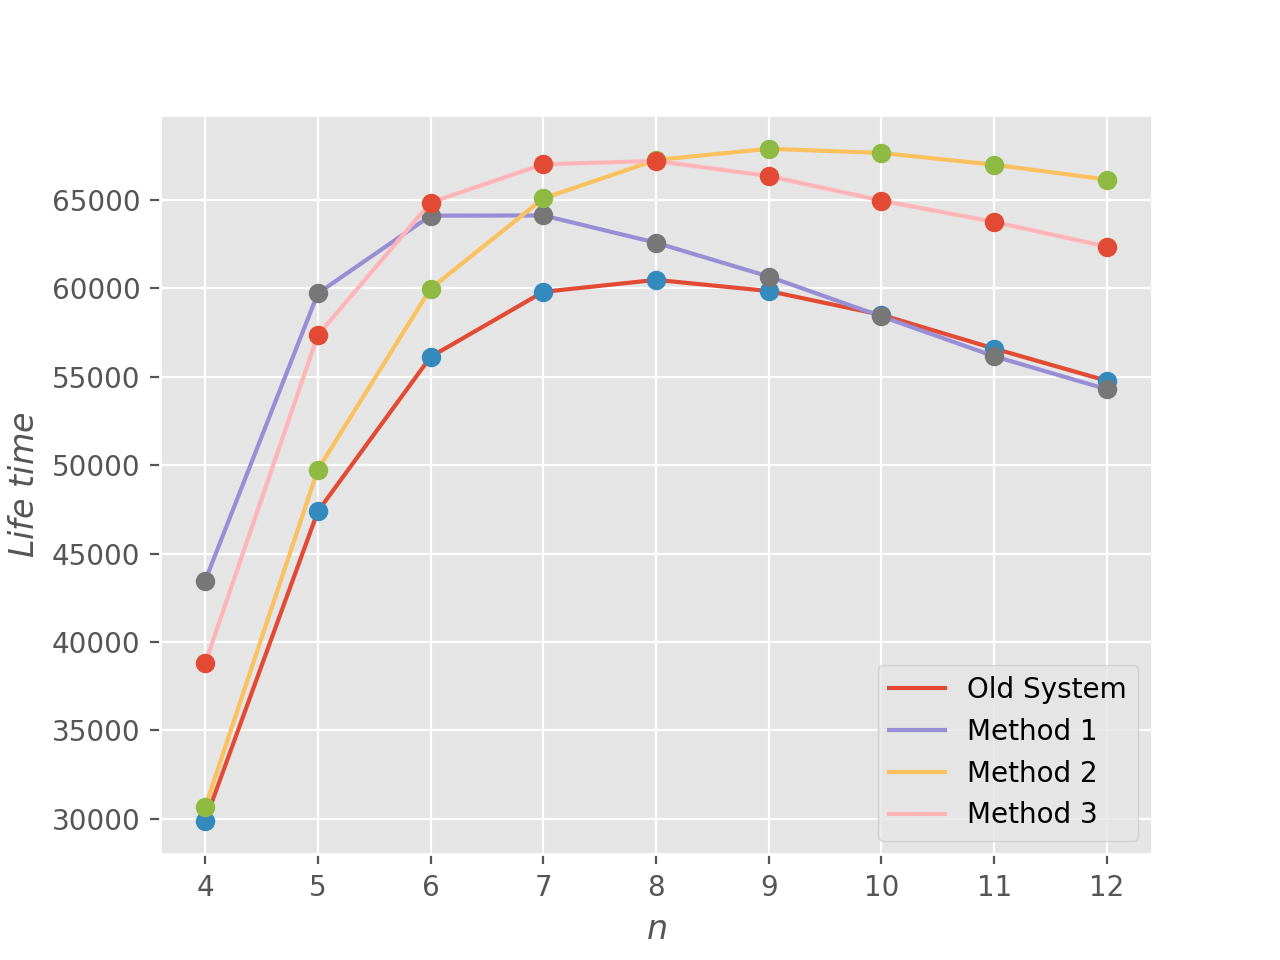
\includegraphics[scale = 0.6]{fig7.png}
	\caption{不同优化方案对应的系统平均寿命和节点个数关系图}
\end{figure}

根据图\ref{fig:7}中不同曲线之间的相对关系,我们得出以系统系统的平均寿命为目标变量的最优方案选择标准。当$n < 6$时,我们应选择升级系统中所有元件中的部件$A$;当$ 6 \leq n \leq 8$时,我们应同时升级系统中所有元件中的部件$A$和部件$B$;当$ n > 8$时,我们应选择升级系统中所有元件的部件$B$。



\renewcommand\refname{\hei\wuhao\centerline{参考文献(References)}\global\def\refname{参考文献}}
\vskip 12pt

\let\OLDthebibliography\thebibliography
\renewcommand\thebibliography[1]{
  \OLDthebibliography{#1}
  \setlength{\parskip}{0pt}
  \setlength{\itemsep}{0pt plus 0.3ex}
}

{
\renewcommand{\baselinestretch}{0.9}
\liuhao
\bibliographystyle{unsrt}
\bibliography{./TempExample}
}
%%%%%!!!!!需要在合适位置插入\newpage,来平衡最后一页两栏!!!!!
\newpage  %%% 用于平衡最后一页两栏高度

%%%%%%%%%%%%%%%%%%%%%%%%%%%%%%%%%%%%%%%%%%%%%%%%%%%%%%%%%%%%%%%
% % % 附录
%%%%%%%%%%%%%%%%%%%%%%%%%%%%%%%%%%%%%%%%%%%%%%%%%%%%%%%%%%%%%%%
\twocolumn[
\begin{@twocolumnfalse}
\vskip 20pt
 
 \noindent {\hei 附录:蒙特卡洛随机模拟算法的代码实现}
 \newline
 \kai (1) 节点(Node)类的设计
\lstinputlisting{Node.m}
\kai (2) 问题求解函数的设计
\lstinputlisting{findresult.m}
\end{@twocolumnfalse}

]

\twocolumn[
\begin{@twocolumnfalse}
\kai(3)蒙特卡洛模拟(Simulation)类的设计
\lstinputlisting{System1.m}
\end{@twocolumnfalse}
]
\twocolumn[
\begin{@twocolumnfalse}
\lstinputlisting{System2.m}

\end{@twocolumnfalse}
]
\twocolumn[
\begin{@twocolumnfalse}
\lstinputlisting{System3.m}

\end{@twocolumnfalse}
]
\twocolumn[
\begin{@twocolumnfalse}
\lstinputlisting{System4.m}

\end{@twocolumnfalse}
]
\twocolumn[
\begin{@twocolumnfalse}
\lstinputlisting{System5.m}

\end{@twocolumnfalse}
]
\twocolumn[
\begin{@twocolumnfalse}
\lstinputlisting{System6.m}

\end{@twocolumnfalse}
]

\end{document}